\documentclass{beamer}
\usepackage{hyperref}
\usepackage{url}
\usepackage{natbib}
\usepackage{xcolor}
\usepackage{graphicx}
%\usepackage{enumitem}  
\usepackage{calc}  
\usepackage{amsmath,amssymb}
\usepackage{amsthm}
\usepackage[ruled,linesnumbered]{algorithm2e}
\usepackage{xspace}


\usepackage{times}
\usepackage{graphicx}
\usepackage{latexsym}
%\usepackage{enumitem}
% \usepackage{algpseudocode}
\usepackage{caption}
\usepackage{subcaption}
\usepackage{float}

\definecolor{vuborange}{rgb}{1.0,0.40,0.0}

% \usepackage{tikz}
%\usetheme{vub} 
% \usetheme{Copenhagen}
\usetheme{Madrid}
\usecolortheme{rose}
%  \usetheme[coloredtitles]{vub}
% \usetheme[showsection]{vub}
\title{Visual Step-By-Step Explanations of Constraint Satisfaction Problems}
\subtitle{ZebraTutor - Explaining logic grid puzzles}
\author{Emilio Gamba\textsuperscript{1}, Bart Bogaerts\textsuperscript{2}, Tias Guns\textsuperscript{1}}
\date{}

\newcommand\m[1]{\ensuremath{#1}\xspace}
\newcommand\allconstraints{\m{T_P}}

\newcommand{\phantomgraphics}[2][]{%
  \leavevmode\phantom{\includegraphics[#1]{#2}}%
}


\makeatletter
\setbeamertemplate{footline}
{
  \leavevmode%
  \hbox{%
  \begin{beamercolorbox}[wd=.333333\paperwidth,ht=2.25ex,dp=1ex,center]{author in head/foot}%
    \usebeamerfont{author in head/foot}Emilio Gamba, Bart Bogaerts, Tias Guns
  \end{beamercolorbox}%
  \begin{beamercolorbox}[wd=.333333\paperwidth,ht=2.25ex,dp=1ex,center]{title in head/foot}%
    \usebeamerfont{title in head/foot}ZebraTutor - XCSP
  \end{beamercolorbox}%
  \begin{beamercolorbox}[wd=.333333\paperwidth,ht=2.25ex,dp=1ex,right]{date in head/foot}%
    \usebeamerfont{date in head/foot}Flanders AI GC4 \hspace*{2em}
    \insertframenumber{} / \inserttotalframenumber\hspace*{2ex} 
  \end{beamercolorbox}}%
  \vskip0pt%
}
\makeatother


\begin{document}

% \begin{frame}{\small{Explainable Artificial Intelligence (XAI)}}
%     \maketitle
% \tiny{\textsuperscript{1}data-lab, Vrije Universiteit Brussel}\\
% \tiny{\textsuperscript{2}AI lab, Vrije Universiteit Brussel}\\
% \tiny{\{firstname.lastname\}@vub.be}
% \end{frame}
% Automatic titlepage with VUB logo.
% \frame{\maketitle}

\begin{frame}
    \maketitle
    \begin{center}
        
    \end{center}
    \tiny{\textsuperscript{1}data-lab, Vrije Universiteit Brussel}\\
    \tiny{\textsuperscript{2}AI lab, Vrije Universiteit Brussel}\\
    \tiny{\{firstname.lastname\}@vub.be}
    % \textbf{Curse of performance}
    % \begin{itemize}
    %     \item Black-box prediction systems (e.g. deep neural networks)
    %     \item Efficient complex reasoning systems with millions of parameters
    % \end{itemize}

    % \begin{figure}[]
    %     \centering
    %     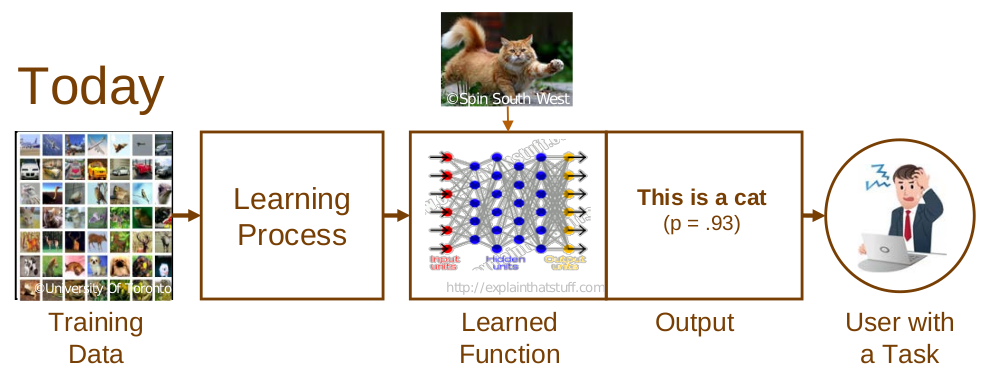
\includegraphics[width=0.8\textwidth]{figures/cat}
    %     {\small \caption{Deep neural network - image classifier \textsuperscript{\cite{gunning2017explainable}}}}
    %     \label{catdog}
    % \end{figure}

\end{frame}

\begin{frame}{\small{Explainable Artificial Intelligence (XAI)}}
    \framesubtitle{Motivation}
    \textbf{Curse of performance}
    \begin{itemize}
        \item Black-box prediction systems (e.g. deep neural networks)
        \item Efficient complex reasoning systems with millions of parameters
    \end{itemize}

    \begin{figure}[]
        \centering
        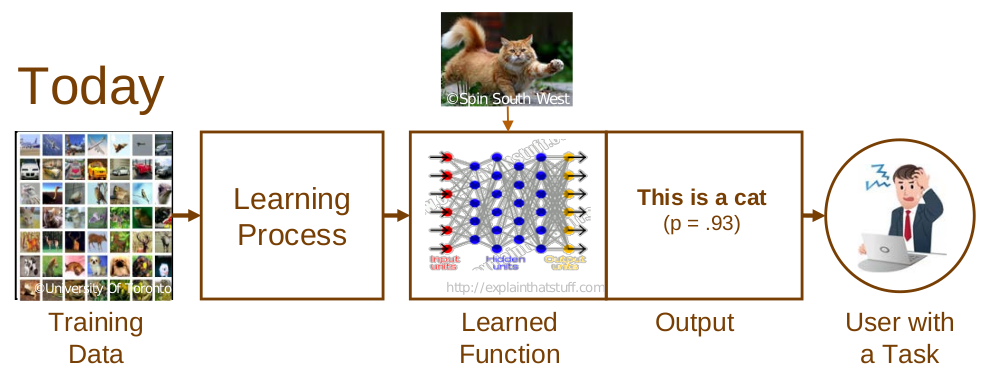
\includegraphics[width=0.8\textwidth]{figures/cat}
        {\small \caption{Deep neural network - image classifier \textsuperscript{\cite{gunning2017explainable}}}}
        \label{catdog}
    \end{figure}

\end{frame}

\begin{frame}{\small{Explainable Artificial Intelligence (XAI)}}
    \framesubtitle{Motivation}
    \begin{block}{Human-interpretability}
        \emph{Users should be able to \textbf{see} but also \textbf{study} and \textbf{understand} how inputs are (mathematically) mapped to outputs.} \textsuperscript{\cite{doran2017does}}
    \end{block}
    \vfill
    % \pause
    \textbf{The A.R.T of Responsible AI \textsuperscript{\cite{adadi2018peeking}}}
    \begin{itemize}
        \item \textbf{\underline{A}ccountability} \textit{need to explain and justify actions to user}
        \item \textbf{\underline{R}esponsibility} \textit{role of answering for one's decisions and identify errors or unexpected results}
        \item \textbf{\underline{T}ransparency} \textit{need to describe, inspect and reproduce AI thought process}
    \end{itemize}
    % \pause
    % \begin{center}
    %     \emph{``XAI is an explanatory agent revealing underlying \textbf{causes} to its or another agent’s decision making''} \textsuperscript{\citep{miller2019explanation}}
    % \end{center}
    % \begin{flushright}
    %     --- Miller, 2019
    % \end{flushright}
\end{frame}


\begin{frame}{\small{Motivation}}



    \begin{itemize}
        \item Our take on explainable AI
        \item Context: Constraint solving
        \item \emph{Explain} (strong, complex) propagation in simple steps
        \item \emph{Interactive} constraint solving
    \end{itemize}

\end{frame}



\begin{frame}{\small{History}}


    2019: \textbf{Holy Grail Challenge - Zebra puzzles}

    \begin{itemize}
        \item Parse puzzles and translate into CSP
        \item Solve CSP automatically
        \item Explain in a \emph{human-understandable} way how to solve this puzzle
    \end{itemize}
    \vspace{1em}
    2020: \textbf{ECAI Accepted paper - formalization of XCSP} \\

    \vspace{1em}

    2020: \textbf{IJCAI Demo - submitted} \\
    \vspace{1em}

    Next: \textbf{AIJournal Special Issue on Explainability} \\
\end{frame}

\begin{frame}{\small{Contributions}}

    \begin{itemize}
        \item Formalize the step-wise explanation problem (ECAI)
              \begin{itemize}
                  \item Propose an algorithm (agnostic of actual propagators, consistency level, etc.)
                  \item Propose heuristics for guiding the search for explanations
                  \item Experimentally demonstrate feasibility
              \end{itemize}
        \item Refine complex explanation steps (nested-explanations, IJCAI, AIJournal)

    \end{itemize}

\end{frame}

%a


% \begin{frame}{\small{Explainable Artificial Intelligence (XAI)}}
%     \framesubtitle{Definition}
%     \vfill

%     \begin{center}
%         \emph{``XAI is an explanatory agent revealing underlying \textbf{causes} to its or another agent’s decision making''} \textsuperscript{\citep{miller2019explanation}}
%     \end{center}
%     \begin{flushright}
%         --- Miller, 2019
%     \end{flushright}
%     \vfill

% \end{frame}

% \begin{frame}{\small{Explaining Constraint Satisfaction Problems}}
%     \framesubtitle{Goal : Explainable agency}
%     \begin{block}{Explainable agency \textsuperscript{\cite{langley2017explainable}}}
%     Given \emph{objectives} and \emph{background knowledge} relevant to objectives:
%     \begin{itemize}
%         \item \small{Produce \emph{records of decision} taken during plan generation}
%         \item \small{Produce summary of agent's \emph{mental effort}}
%         \item \small{Produce \emph{understandable explanations} about specific choices and reasons for them}
%     \end{itemize}
%     \end{block}
%     \begin{figure}[]
%         \centering
%         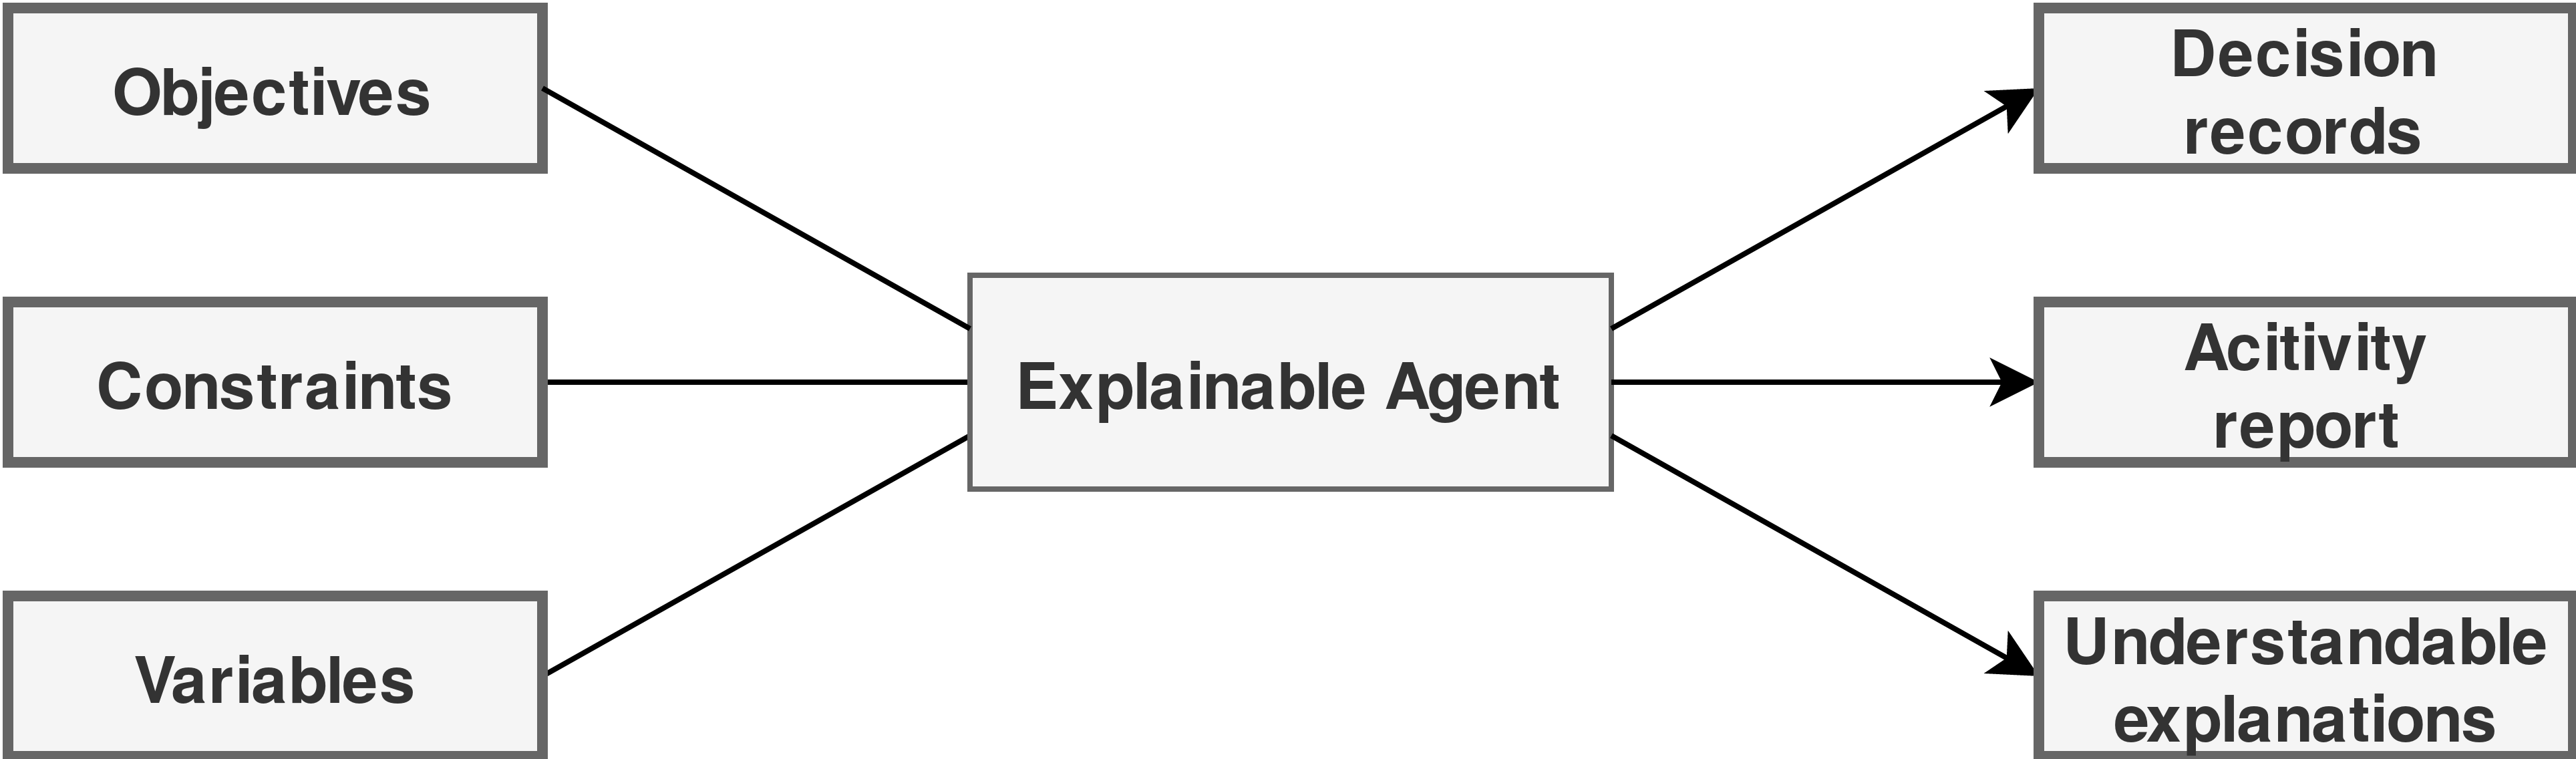
\includegraphics[width=0.7\textwidth]{figures/explainable_agency2}
%     \end{figure}


% \end{frame}


\begin{frame}{\small{Explaining Constraint Satisfaction Problems}}
    \framesubtitle{ZebraTutor : an \emph{explainable} agent }

    \only<1>{
        % \begin{block}{Explainable agency\textsuperscript{\cite{langley2017explainable}} - Problem statement }
        %     Given the natural language problem statement and set of clues (entities, constraints)
        % \end{block}
        \vfill
        \begin{figure}[]
            \centering
            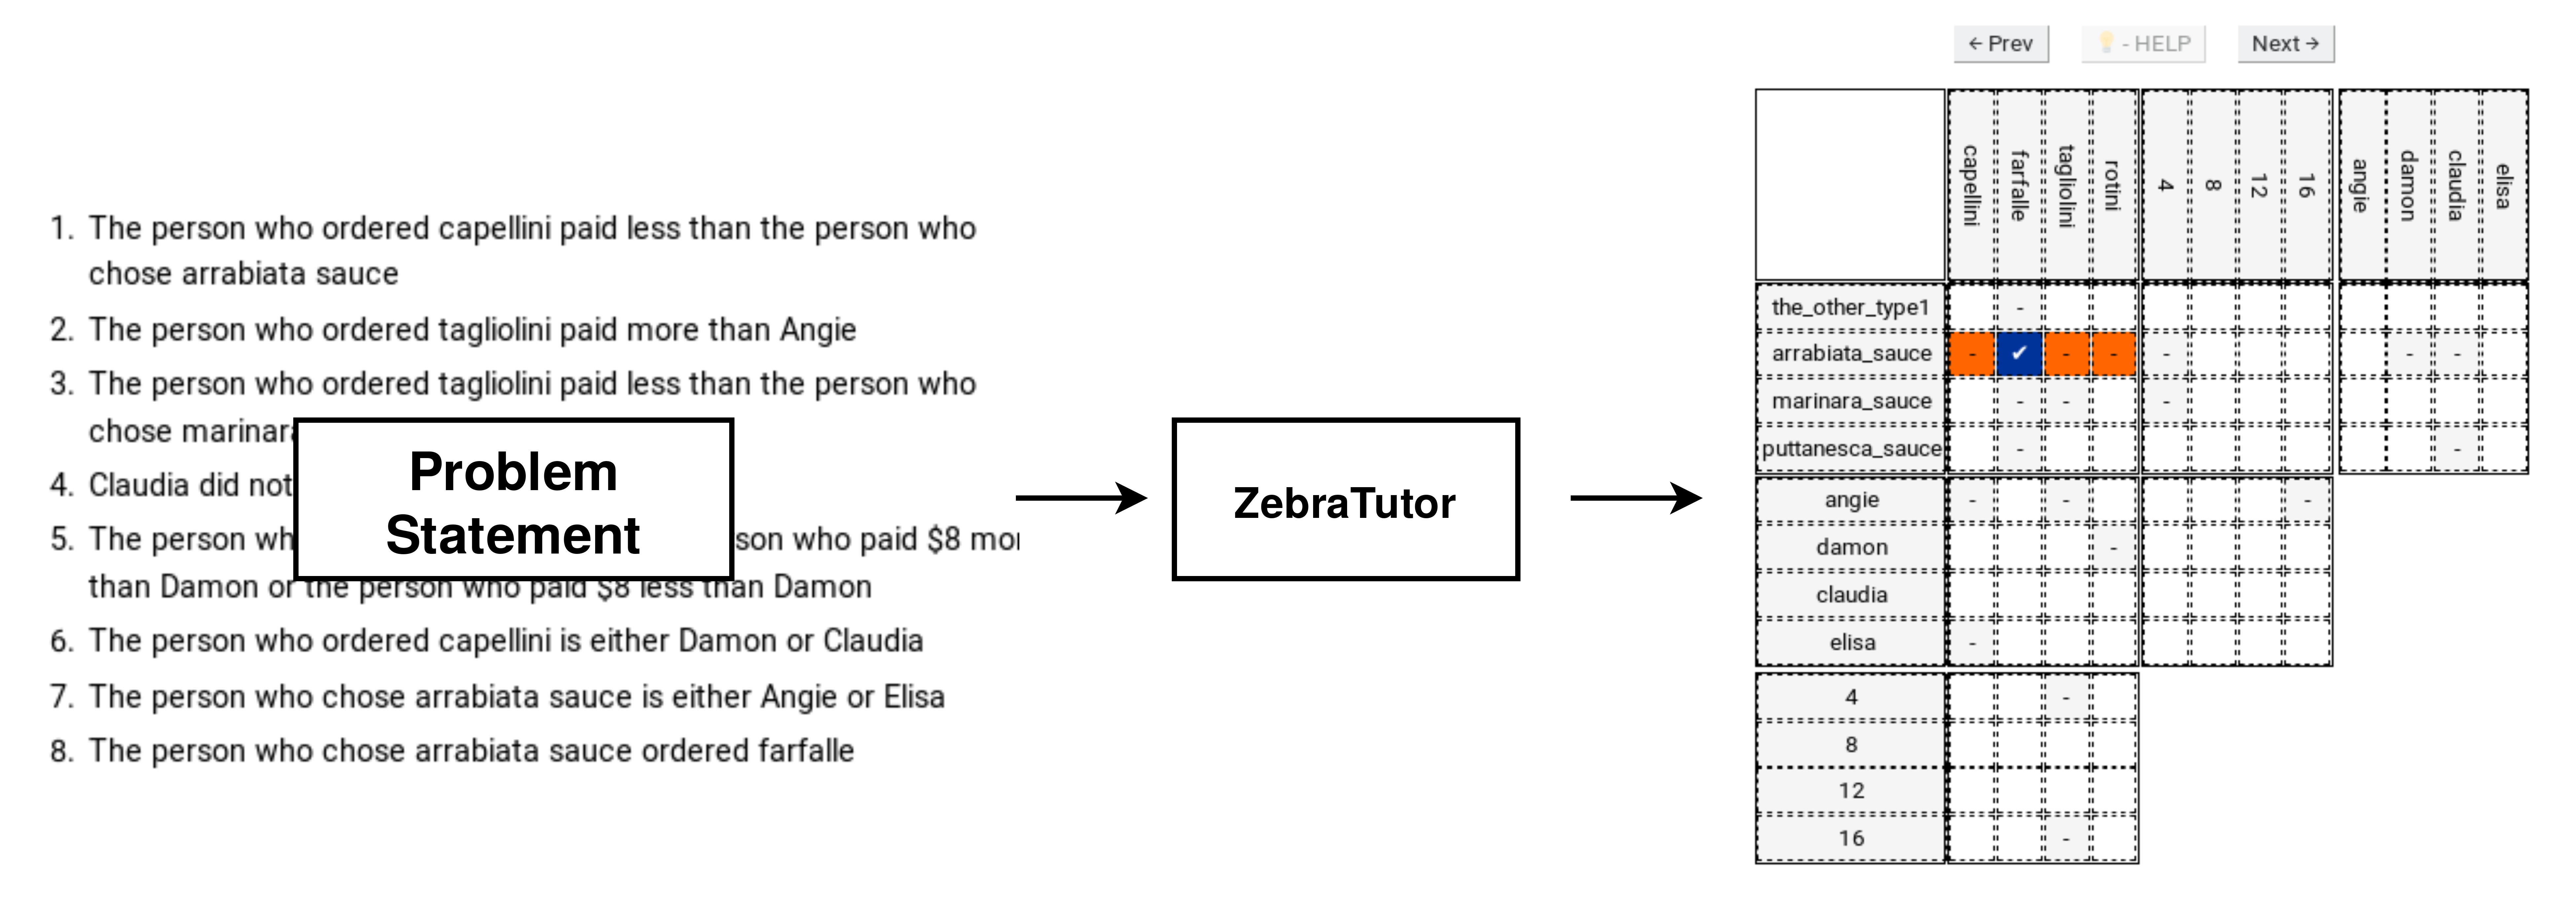
\includegraphics[width=\textwidth]{figures/puzzle_pipeline_4}
        \end{figure}
    }
    \pause
    \only<2>{
        \begin{block}{Explainable agency\textsuperscript{\cite{langley2017explainable}} - Problem statement }
            Given the natural language problem statement and set of clues (entities, constraints):
            \begin{itemize}
                \item Produce the \emph{explanation sequence} to solve the puzzle
                      \phantom{\parbox{\linewidth}{\item Produce the cost (mental effort) associated to each step}}
                      \phantom{\parbox{\linewidth}{\item Produce the \emph{cognitively-easiest explanation} for each step in the explanation sequence}}
            \end{itemize}
        \end{block}
        \begin{figure}[]
            \centering
            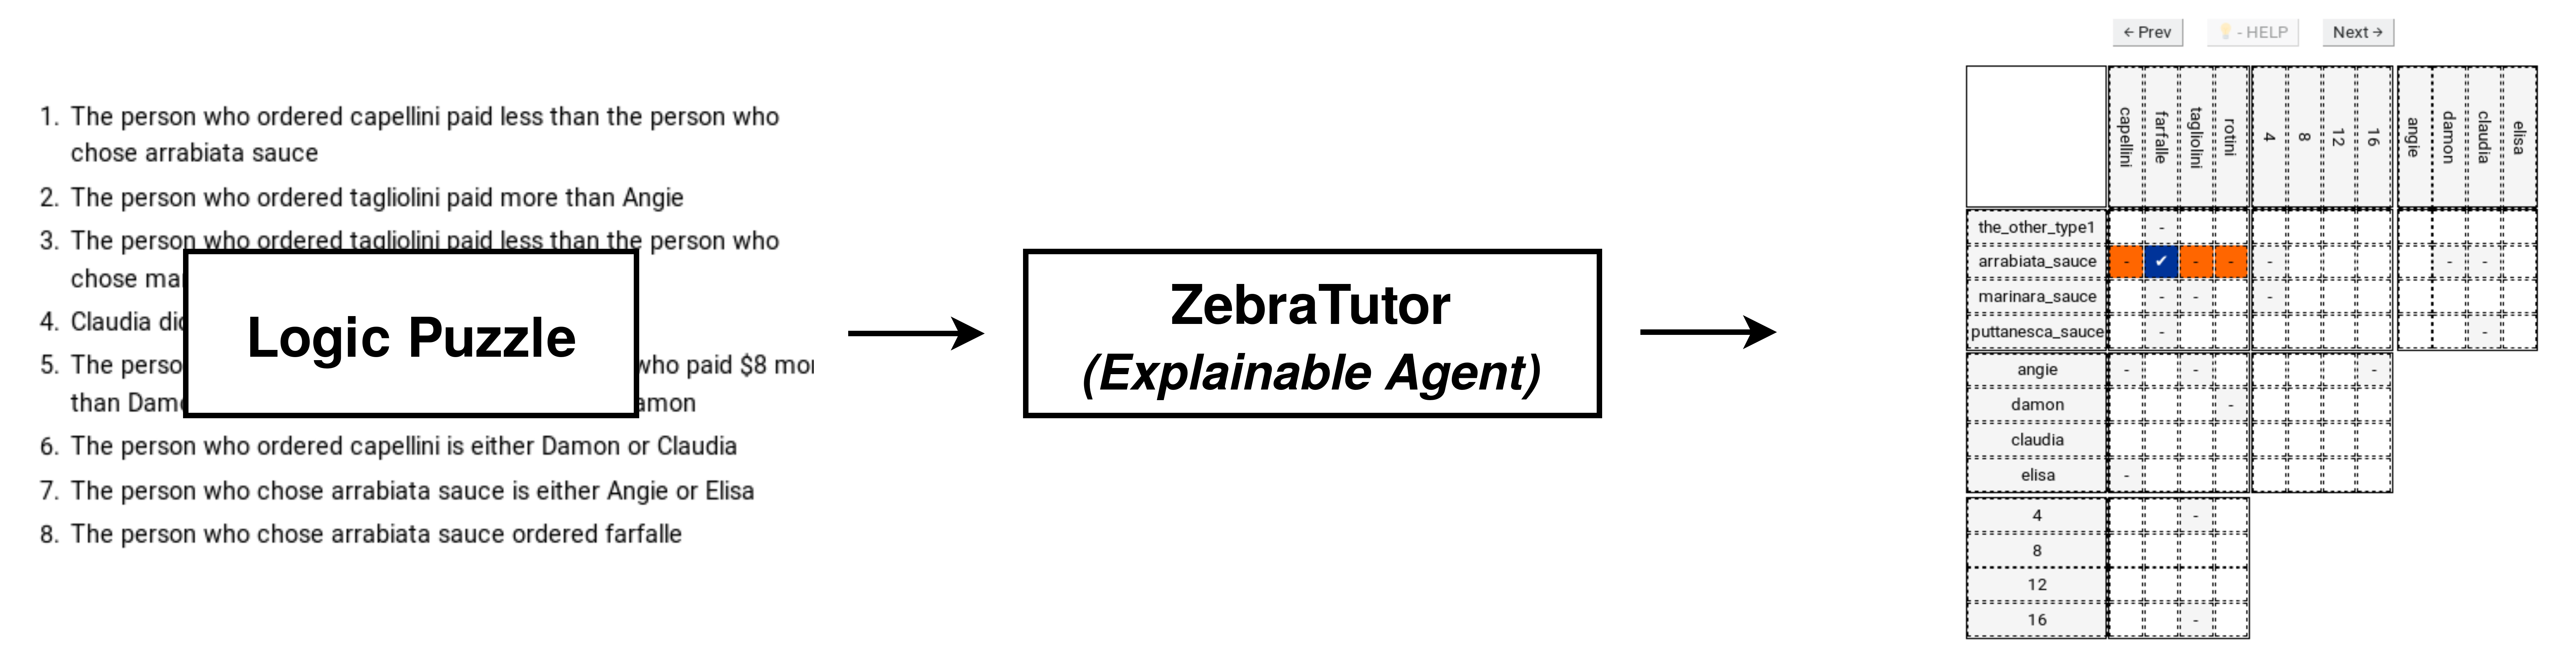
\includegraphics[width=0.8\textwidth]{figures/puzzle_pipeline}
        \end{figure}
    }

    \pause
    \only<3>{
        \begin{block}{Explainable agency\textsuperscript{\cite{langley2017explainable}} - Problem statement}
            Given the natural language problem statement and set of clues (entities, constraints):
            \begin{itemize}
                \item Produce the \emph{explanation sequence} to solve the puzzle
                \item Produce the cost (mental effort) associated to each step
                      \phantom{\parbox{\linewidth}{\item Produce the \emph{cognitively-easiest explanation} for each step in the explanation sequence}}
            \end{itemize}
        \end{block}
        \begin{figure}[]
            \centering
            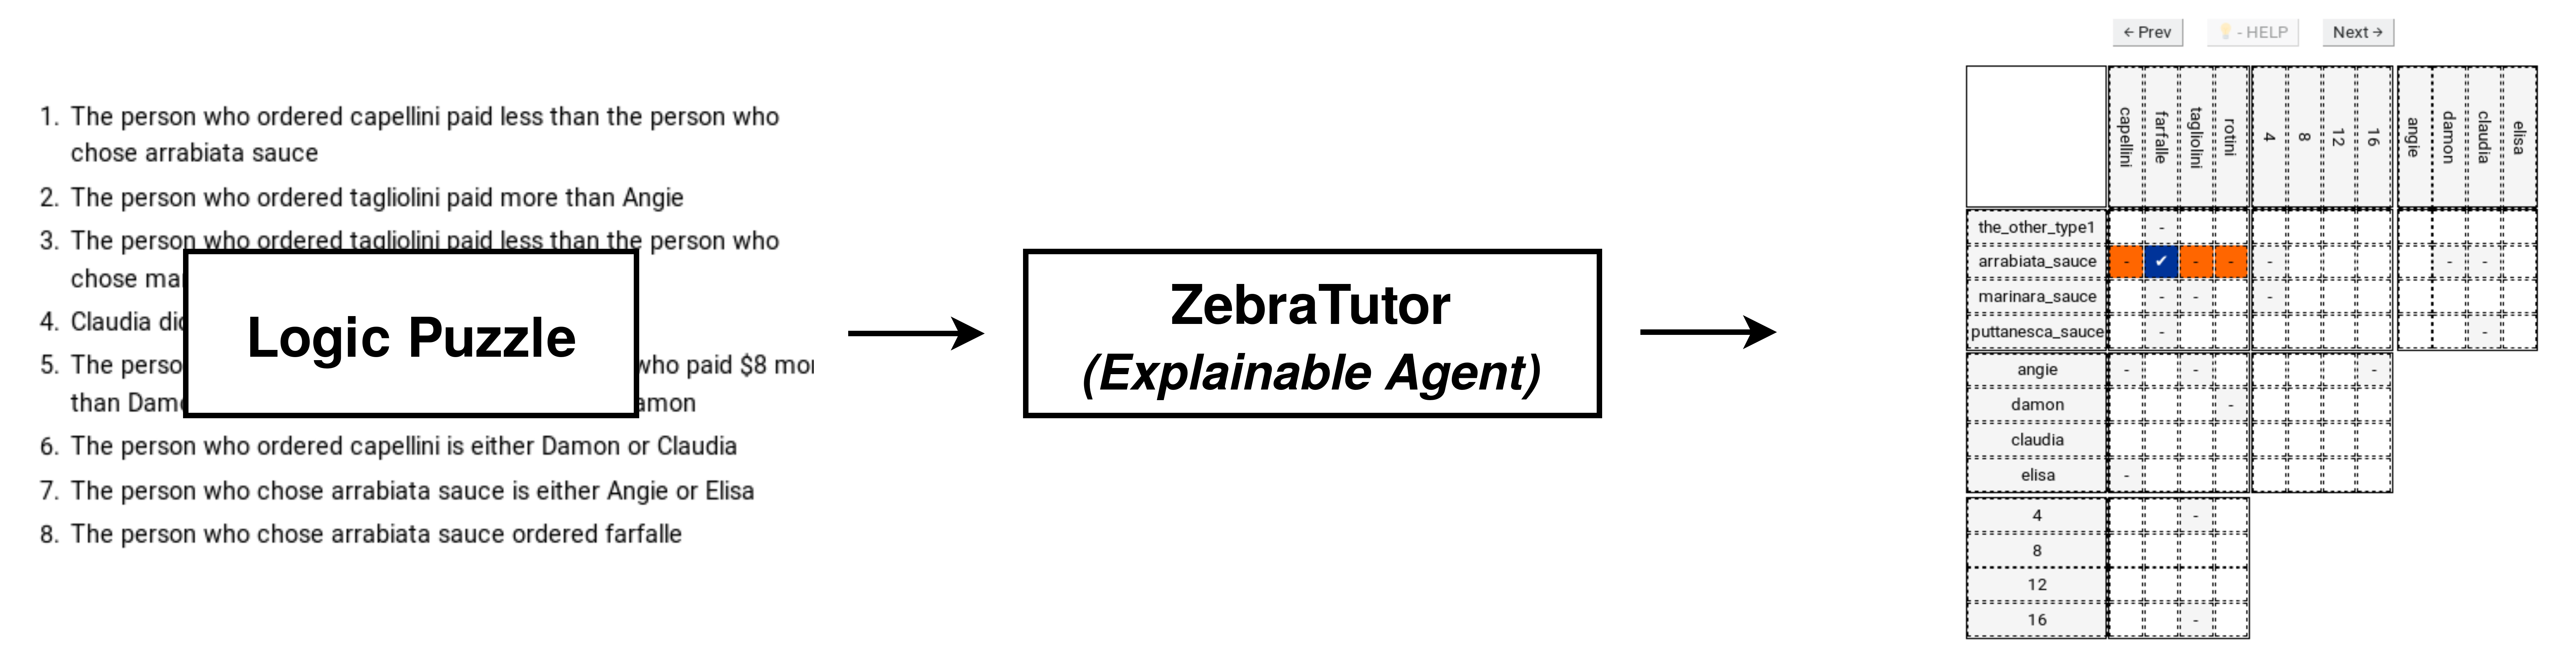
\includegraphics[width=0.8\textwidth]{figures/puzzle_pipeline}
        \end{figure}
    }

    \pause
    \only<4>{
        \begin{block}{Explainable agency\textsuperscript{\cite{langley2017explainable}} - Problem statement}
            Given the natural language problem statement and set of clues (entities, constraints):
            \begin{itemize}
                \item Produce the \emph{explanation sequence} to solve the puzzle
                \item Produce the cost (mental effort) associated to each step
                \item Produce the \emph{cognitively-easiest explanation} for each step in the explanation sequence
            \end{itemize}
        \end{block}
        \begin{figure}[]
            \centering
            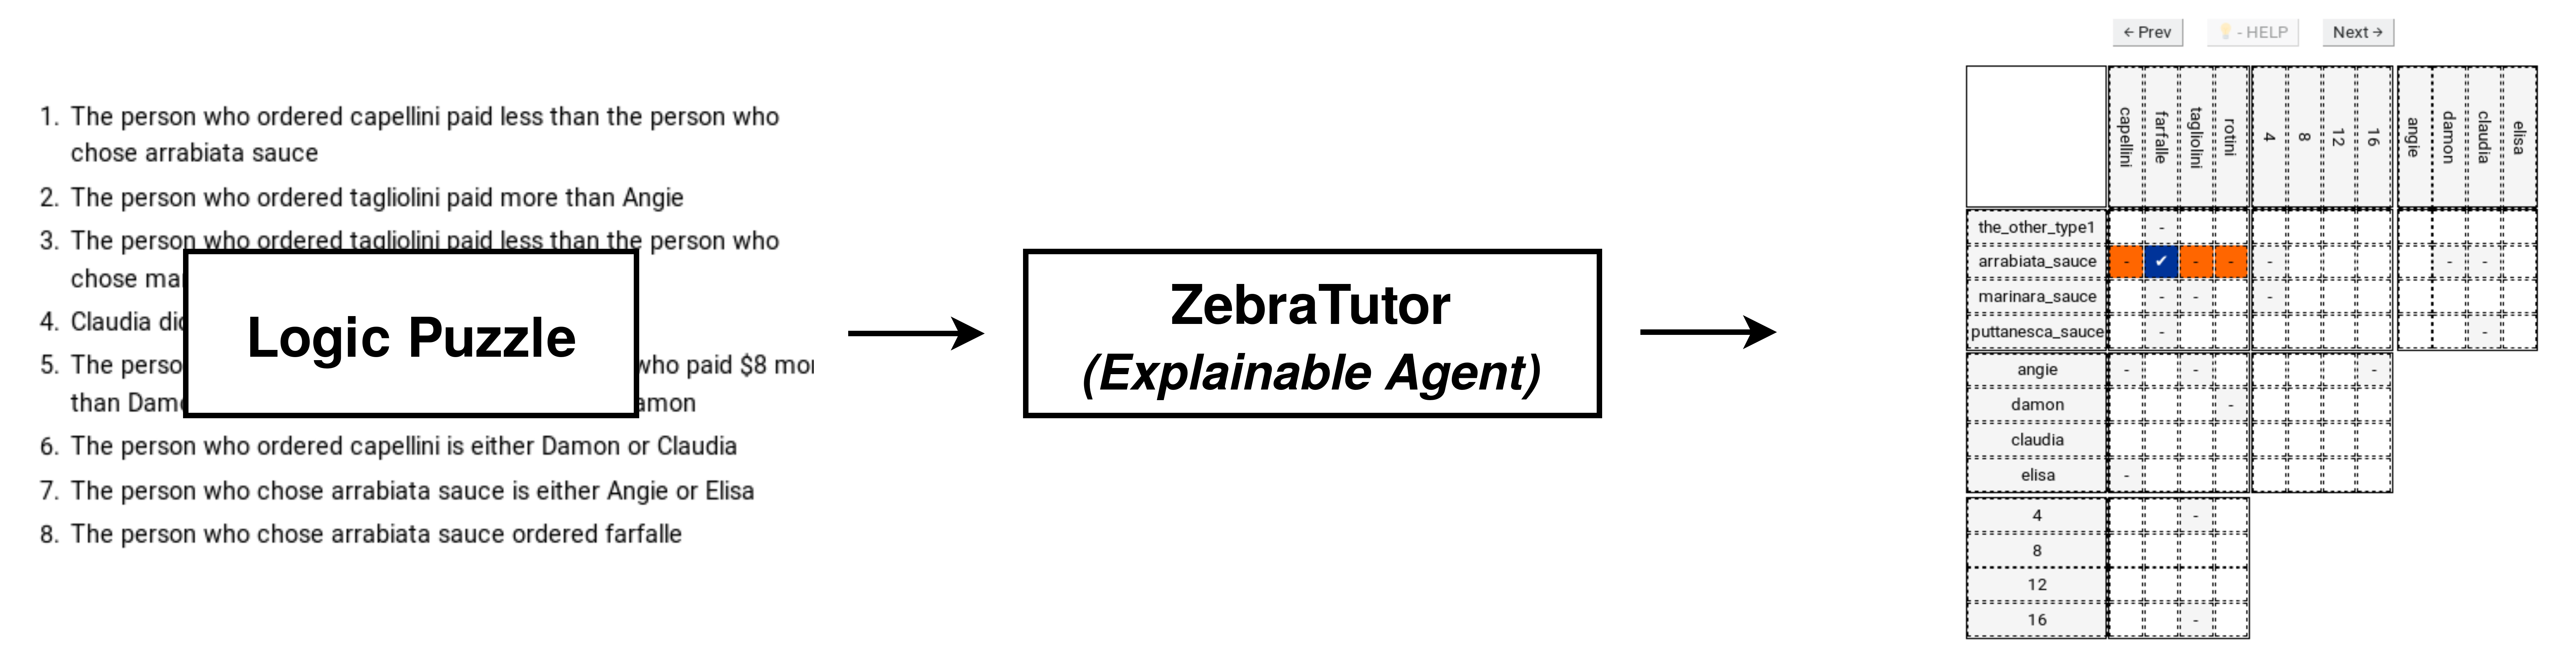
\includegraphics[width=0.8\textwidth]{figures/puzzle_pipeline}
        \end{figure}
    }

    % \vfill


\end{frame}

\begin{frame}{\small{Explaining Constraint Satisfaction Problems}}
    \framesubtitle{ZebraTutor : an \emph{explainable} agent }
    % \vspace{1cm}
    % \only<1>{
    %     \begin{block}{Problem statement}
    %         Given the natural language problem statement and set of clues (entities, constraints):
    %         \begin{itemize}
    %             \item Produce the \emph{explanation sequence} to solve the puzzle
    %             \item Produce the cost (mental effort) associated to each step
    %             \item Produce the \emph{cognitively-easiest explanation} for each step in the explanation sequence
    %         \end{itemize}
    %     \end{block}
    %     \phantomgraphics[width=\textwidth]{figures/step_1}%
    % }
    % \only<8>{

    % }
    % \vfill
    % \pause
    % \only<1-8>{
    \begin{block}{\textcolor{lightgray}{Problem statement}}
        \textcolor{lightgray}{
            Given the natural language problem statement and set of clues (entities, constraints):}
        \begin{itemize}
            \item \textcolor{lightgray}{Produce the \textcolor{black}{\emph{explanation sequence}} to solve the puzzle}
            \item \textcolor{lightgray}{Produce the cost (\textcolor{black}{mental effort}) \textcolor{black}{associated to each step}}
            \item \textcolor{lightgray}{Produce the \textcolor{black}{\emph{cognitively-easiest explanation}} for each step in the explanation sequence}
        \end{itemize}
    \end{block}
    % }
    % \only<1>{\begin{figure}[]
    %         \centering
    %         
\includegraphics[width=\textwidth]{figures/step_1}
    %     \end{figure}}
    % \pause
    % \only<2>{\begin{figure}[]
    %         \centering
    %         
\includegraphics[width=\textwidth]{figures/step_2}
    %     \end{figure}}
    % \pause
    % \only<3>{\begin{figure}[]
    %         \centering
    %         
\includegraphics[width=\textwidth]{figures/step_3}
    %     \end{figure}}
    % \pause
    % \only<4>{\begin{figure}[]
    %         \centering
    %         
\includegraphics[width=\textwidth]{figures/step_4}
    %     \end{figure}}
    % \pause
    % \only<5>{\begin{figure}[]
    %         \centering
    %         
\includegraphics[width=\textwidth]{figures/step_5}
    %     \end{figure}}
    % \pause
    % \only<6>{\begin{figure}[]
    %         \centering
    %         
\includegraphics[width=\textwidth]{figures/step_6}
    %     \end{figure}}
    % \pause
    % \only<7>{\begin{figure}[]
    %         \centering
    %         
\includegraphics[width=\textwidth]{figures/step_7}
    %     \end{figure}}
    % \pause
    % \only<8>{

    \begin{figure}[]
        \centering
        
\includegraphics[width=\textwidth]{figures/step_8}
    \end{figure}
    % }

\end{frame}

\begin{frame}{\small{Explaining Constraint Satisfaction Problems}}
    \frametitle{Demo}

    \begin{center}
        {\Large \url{https://bartbog.github.io/zebra/pasta/}}
    \end{center}
    

\end{frame}

\begin{frame}{\small{Explaining Constraint Satisfaction Problems}}
    \framesubtitle{ZebraTutor : background}
    % \vspace{1.5cm}
    \begin{block}{Typed Entity} \textit{Elisa} \texttt{[Person]}, \textit{farfalle} \texttt{[Pasta]}\end{block}
    \vspace{0.5em}
    \begin{block}{Literal} relation between entities $chose(Elisa, farfalle)$\end{block}
    \vspace{0.5em}
    \begin{block}{Clue}A clue is a first-order logic theory $\allconstraints$
        \begin{center}
            ``\emph{The person who chose arrabiata sauce ordered farfalle}''\\
            \vspace{0.5em}
            $\exists$ p \texttt{[Person]} : chose(p, arrabiata) $\wedge$ ordered(p, farfalle)
        \end{center}
    \end{block}

\end{frame}

\begin{frame}{\small{Explaining Constraint Satisfaction Problems}}
    \framesubtitle{ZebraTutor : csp problem definition}
    \vfill
    \textbf{Goal} Find relations between each two types s.t.:
    {\small
    \begin{itemize}
        \item Each clue is respected
        \item \textbf{Bijectivity} Entity of 1 type is matched exactly with 1 entity of the second type (reverse holds)
        \item \textbf{Transitivity} Relations are logically linked:\\
              ``If Angie chose arrabiata sauce, and arrabiata sauce is paired with farfalle, then Angie must have eaten farfalle''
    \end{itemize}
    }

\end{frame}


% \begin{frame}{\small{Explaining Constraint Satisfaction Problems}}
%     \framesubtitle{ZebraTutor : background}
%     % \vspace{1.5cm}
%     \begin{block}{(Partial) Interpretation}
%         Finite set of literals of the form $P(\overline{d})$ or $\neg P(\overline{d})$
%         \begin{description}
%             \item[$P$] {\small where  is a relation symbol typed $T_1 \times ... \times T_n$}
%             \item[$\overline{d}$] {\small where  is tuple of domain elements, $d_i$ is of type $T_i$}
%             \item[$I_1$] $\{chose(Elisa, farfalle), \neg chose(Angie, farfalle) \}$
%         \end{description}
%     \end{block}
%     \begin{block}{Full Interpretation $I$}
%         I contains $P(\overline{d})$ or $\neg P(\overline{d})$ for each well-typed atom $P(\overline{d})$
%     \end{block}

%     \begin{block}{$I_2 \geq_p I_1$}
%         Interpretation $I_2$ is more precise than $I_1$  iff $I_2$ contains at least all the literals of $I_1$
%     \end{block}
% \end{frame}

\begin{frame}{\small{Explaining Constraint Satisfaction Problems}}
    \framesubtitle{ZebraTutor : background}
    % \vspace{1.5cm}
    \begin{block}{(Partial) Interpretation}
        Finite set of literals of the form $P(\overline{d})$ or $\neg P(\overline{d})$
        \begin{description}
            \item[$P$] {\small where  is a relation symbol typed $T_1 \times ... \times T_n$}
            \item[$\overline{d}$] {\small where  is tuple of domain elements, $d_i$ is of type $T_i$}
            \item[$I_1$] $\{chose(Elisa, farfalle), \neg chose(Angie, farfalle) \}$
        \end{description}
    \end{block}

    \begin{block}{Sequence of incremental partial interpretations}
        A \textit{sequence of incremental partial interpretations} of a theory $\allconstraints$ with initial partial interpretation $I_0$ is a sequence $\langle I_0, I_1, \ldots, I_n  = max(I_0,\allconstraints)\rangle$ where $\forall i>0, I_{i-1} \leq_p I_{i}$ (i.e., the sequence is precision-increasing).
    \end{block}
    % \begin{block}{Full Interpretation $I$}
    %     I contains $P(\overline{d})$ or $\neg P(\overline{d})$ for each well-typed atom $P(\overline{d})$
    % \end{block}

    % \begin{block}{$I_2 \geq_p I_1$}
    %     Interpretation $I_2$ is more precise than $I_1$  iff $I_2$ contains at least all the literals of $I_1$
    % \end{block}
\end{frame}


% \begin{frame}{\small{Explaining Constraint Satisfaction Problems}}
%     \framesubtitle{ZebraTutor : background}
%     % \vspace{1.5cm}

%     % \begin{block}{Full Interpretation $I$}
%     %     I contains $P(\overline{d})$ or $\neg P(\overline{d})$ for each well-typed atom $P(\overline{d})$
%     % \end{block}

%     \begin{block}{Maximal consequence max($I$, $\allconstraints$)}
%         The \textit{maximal consequence  of a theory $\allconstraints$}, and \textit{partial interpretation I},  $J$ is the precision-maximal partial interpretation J s.t. $I \wedge \allconstraints \models J$
%     \end{block}

%     \begin{block}{Sequence of incremental partial interpretations}
%         A \textit{sequence of incremental partial interpretations} of a theory $\allconstraints$ with initial partial interpretation $I_0$ is a sequence $\langle I_0, I_1, \ldots, I_n  = max(I_0,\allconstraints)\rangle$ where $\forall i>0, I_{i-1} \leq_p I_{i}$ (i.e., the sequence is precision-increasing).
%     \end{block}

% \end{frame}

% \begin{frame}{\small{Explaining Constraint Satisfaction Problems}}
%     \framesubtitle{ZebraTutor : background (2)}

%     A sequence $\langle I_0, I_1, ..., I_n = max(I, \allconstraints)\rangle$ where 

% \end{frame}

\begin{frame}{\small{Explaining Constraint Satisfaction Problems}}
    \framesubtitle{ZebraTutor : Explanation-Producing Problem}
    \begin{block}{Explanation $(E,S,N)$}
        Let $I_{i-1}$ and $I_i$ be partial interpretations such that $I_{i-1}\wedge T \models I_i$.
        We say that $(E_i,S_i,N_i)$ \emph{explains} the derivation of $I_{i}$ from $I_{i-1}$ if the following hold:
        \begin{itemize}
            \item $N_i= I_i \setminus I_{i-1}$ (i.e., $N_i$ consists of all newly defined facts),
            \item $E_i\subseteq I_i$ (i.e., the explaining facts are a subset of what was previously derived),
            \item $S_i \subseteq T_P$ (i.e., a subset of the clues and implicit constraints are used), and
            \item $S_i \cup E_i \models N_i$ (i.e., all newly derived information indeed follows from this explanation).
        \end{itemize}
    \end{block}
\end{frame}

\begin{frame}{\small{Explaining Constraint Satisfaction Problems}}
    \framesubtitle{ZebraTutor : Explanation-Producing Problem}
    \begin{block}{Non-redundant explanation}
        We call $(E_i,S_i,N_i)$ a \emph{non-redundant explanation of  the derivation of $I_i$ from $I_{i-1}$} if it explains this derivation and whenever $E'\subseteq E_i; S'\subseteq S_i$ while $(E',S',N_i)$ also explains this derivation, it must be that $E_i=E', S_i=S'$.
    \end{block}
    \pause
    Furthermore, we assume existence of a \emph{cost function} $f(E_i,S_i,N_i)$ that quantifies the interpretability of a single explanation
\end{frame}


\begin{frame}{\small{Explaining Constraint Satisfaction Problems}}
    \framesubtitle{ZebraTutor : Explanation-Producing Problem}
    \begin{definition}
        Given a theory $T$ and initial partial interpretation $I_0$, the \emph{explanation-production problem} consist of finding a non-redundant explanation sequence
        \[ \langle (I_0,(\emptyset,\emptyset,\emptyset)), (I_1,(E_1,S_1,N_i)), \dots ,(I_n,(E_n,S_n,N_n)) \rangle\]
        such that a predefined aggregate over the sequence $\left(f(E_i,S_i,N_i)\right)_{i\leq n}$ is minimised.
    \end{definition}
\end{frame}

\begin{frame}
    \frametitle{\small{Explaining Constraint Satisfaction Problems}}
    \framesubtitle{ZebraTutor : Explanation-Producing Problem}

    \textbf{Algorithm}
    \begin{itemize}
        \item Greedy algorithm (max aggregate)
        \item Prune based on optimistic approximation of cost
        \item Finding non-redundant explanations : Unsat-core extraction (IDP system)
    \end{itemize}

\end{frame}

% \begin{frame}
%     \frametitle{\small{Explaining Constraint Satisfaction Problems}}
%     \framesubtitle{ZebraTutor : Explanation-Producing Problem}

%     \begin{center}
%         \begin{minipage}{0.77\linewidth}
%             \begin{algorithm}[H]
%                 \DontPrintSemicolon
%                 $I_{end} \gets$ propagate$(I_0\land T_p)$\;
%                 Seq $\gets \langle \emptyset \rangle$ \;
%                 $I \gets I_0$\;
%                 \While{$I \neq I_{end}$}{
%                     $(E, S, N) \gets $min-explanation$(I, T_p)$\;
%                     {\color{vuborange}
%                     $nested \gets $ nested-explanation(E, S, N)\;
%                     \uIf{$nested \neq \emptyset$}{
%                         append $nested$ to Seq\;}
%                     \Else{
%                         append $(E, S, N)$ to Seq\;
%                     }
%                     }
%                     $I \gets I \cup N$\;
%                 }
%                 \caption{\small Greedy sequence-generating algorithm.}
%             \end{algorithm}
%         \end{minipage}%
%     \end{center}
% \end{frame}

\begin{frame}
    \frametitle{\small{Explaining Constraint Satisfaction Problems}}
    \textbf{Use cases}
    \begin{itemize}
        \item Teach humans how to solve a certain problem
        \item Quantify problem difficulty
        \item “Help” button
        % \item Interactive configuration/planning/scheduling
    \end{itemize}

\end{frame}

\begin{frame}
    \frametitle{\small{Future Perspectives}}

    \begin{itemize}
        \item Extend explanation capacity to constraint optimization problems
        \item Fast explanation generation: Unsat-core optimization
        \item Learning cost/optimization function
        \item Interactive configuration/planning/scheduling
    \end{itemize}

\end{frame}



\bibliographystyle{abbrv}
\begin{frame}
    \frametitle{References}
    \vspace{2em}
    \bibliography{references}
\end{frame}

\end{document}